\documentclass{article}

\usepackage{summary}

\subject{Informationsgestützte Modellierung von Organisationen}
\semester{Summer 2024}
\author{Leopold Lemmermann}

\begin{document}\createtitle

\part{Modellierung \& Simulation}

\section{Grundbegriffe}
\begin{figure}
  \centering
  \resizebox{0.5\textwidth}{!}{%
    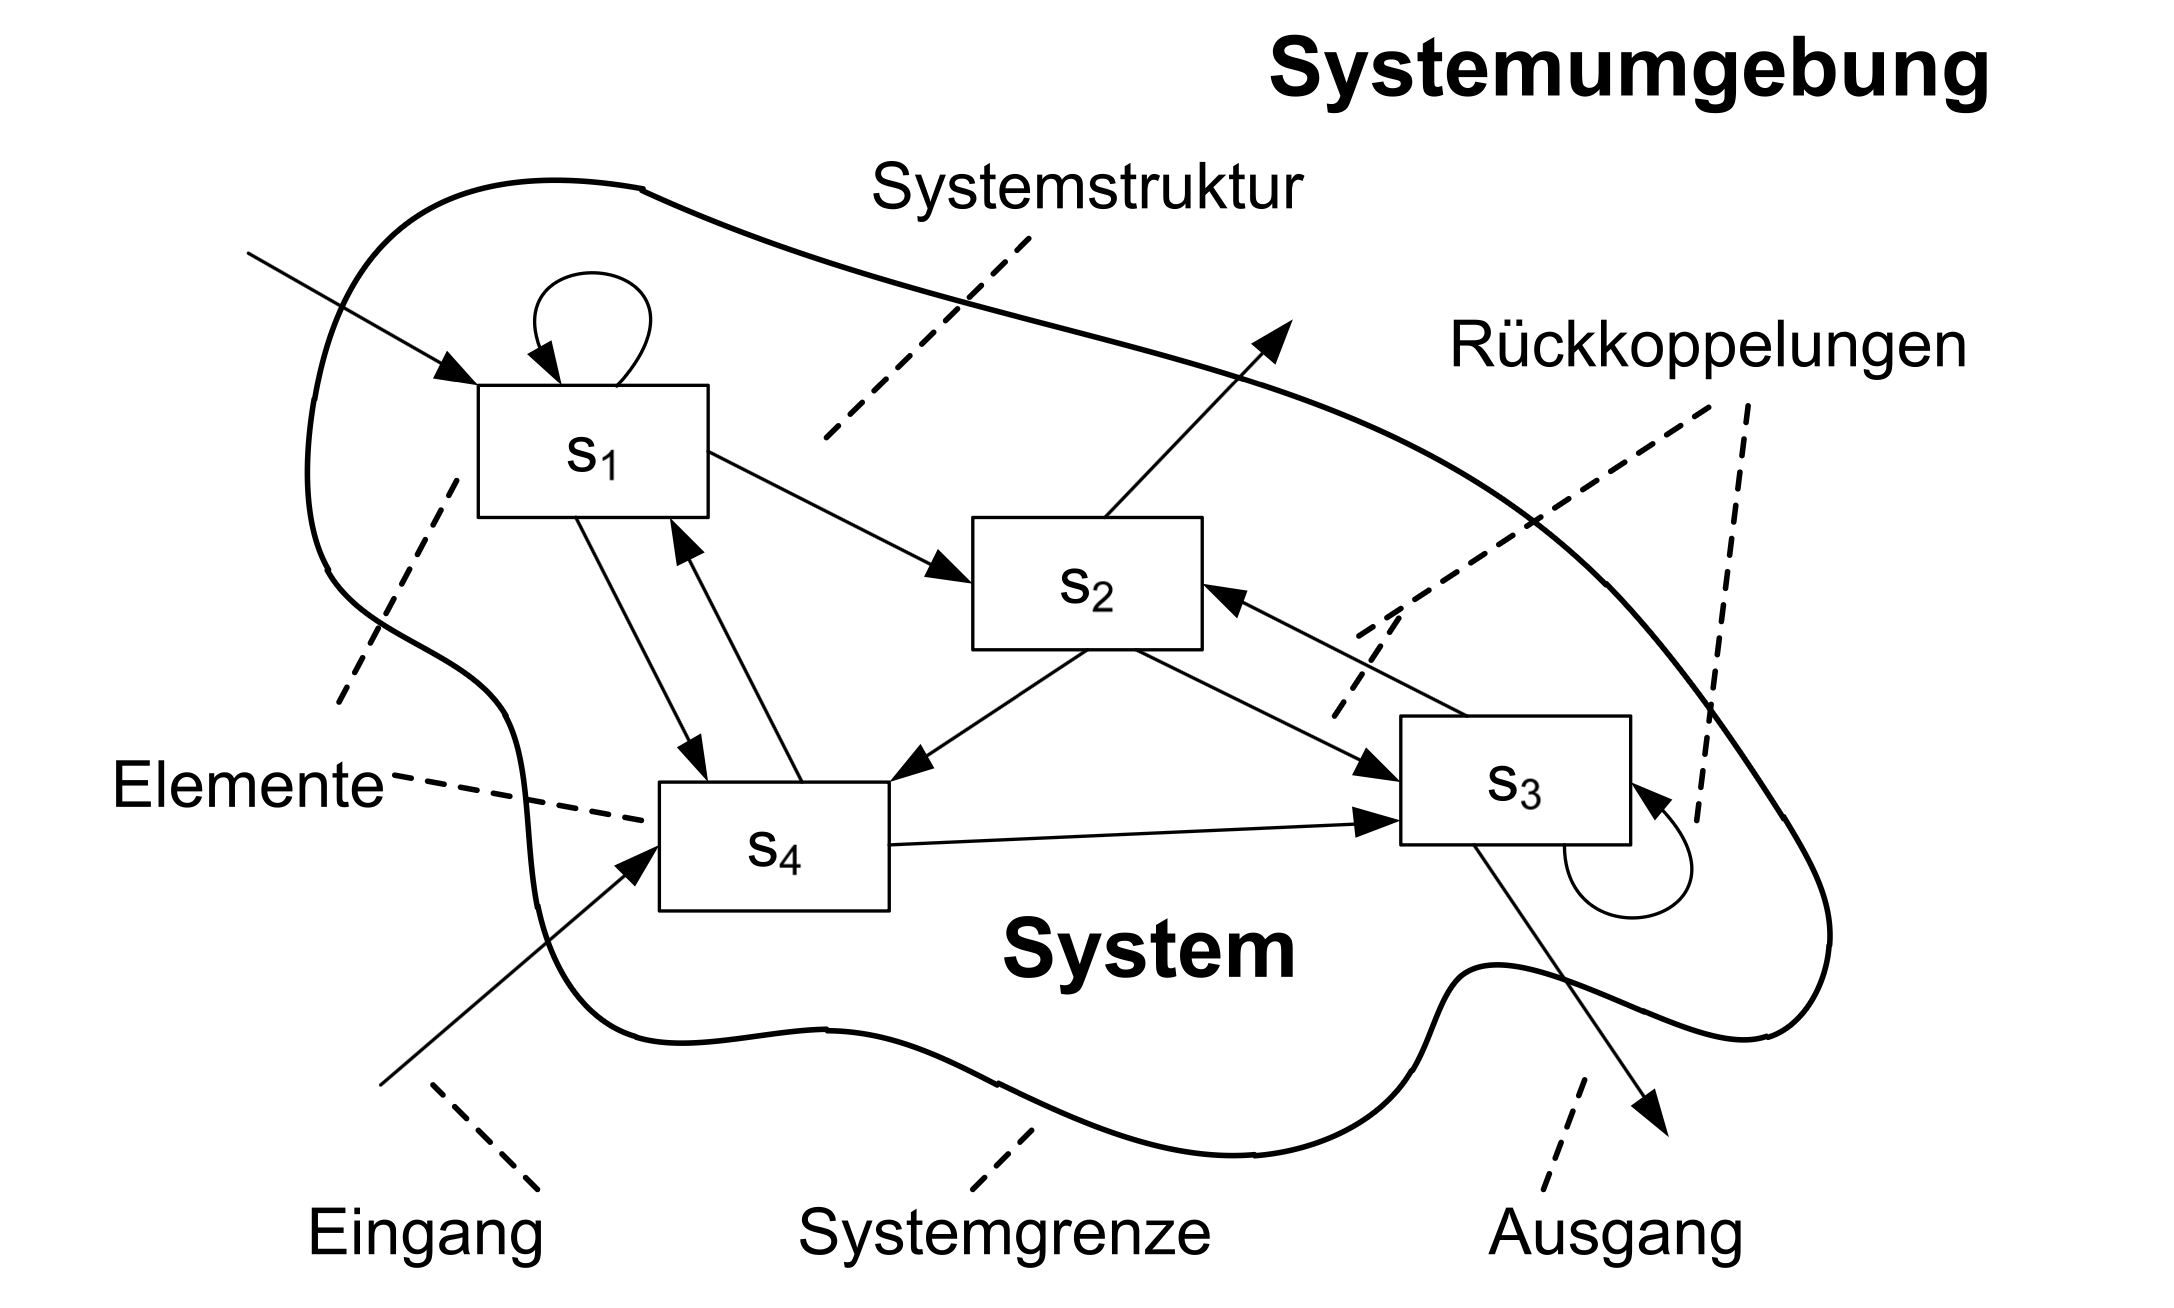
\includegraphics{res/system.png}
  }
  \caption{System}
\end{figure}

\begin{itemize}
  \item \textbf{System}: Ausschnitt aus Gesamtmenge der Objekte \& Beziehunge
  \item \textbf{Systemtheorie}: Erforschung allgemeiner Prinzipien von Systemen
  \item \textbf{Objekt}: (auch Element) kleinste Komponenten eines Systems
  \item \textbf{Zustand}: Menge der Eigenschaften/Zustandsvariablen zu einem Zeitpunkt
  \item \textbf{Verhalten}: dynamische Zustandsfolgen
\end{itemize}

\subsection{Charakteristika}
\begin{itemize}
  \item \textbf{Komplexität}: Anzahl der Elemente, Beziehungen, Zustände
  \item \textbf{Offenheit}: Austausch mit Umwelt
  \item \textbf{Dynamik}: ($\not\leftrightarrow$ Statik) Veränderung über Zeit
  \item \textbf{Kybernetik}: Berücksichtigung von Rückkopplungen
\end{itemize}

\subsection{Modellierung}
\begin{quote}vereinfachende Abbildung (Occam's Razor) eines Systems: \textit{More an art, than a science!}\end{quote}

\begin{itemize}
  \item \textbf{Abstraktion}: Weglassen von Details
  \item \textbf{Idealisierung}: Außerachtlassen von Unerwünschtem \& Irrationalem
\end{itemize}

\subsubsection{Motivationen mit Beispiel}
\begin{itemize}
  \item \textbf{Erklärung}: Stadtplan
  \item \textbf{Prognose}: Wettervorhersage
  \item \textbf{Gestaltung}: Flugzeugdesign
  \item \textbf{Optimierung}: Produktionsplanung
\end{itemize}

\subsection{Simulation}
\begin{quote}Nachahmung von Experimenten an Modellen.\end{quote}

\begin{table}
  \centering
  \begin{tabular}{c|c}
    Vorteile                         & Nachteile \\
    \hline
    \begin{minipage}{0.45\textwidth}
      \begin{itemize}
        \item Realitätsnähe (weniger Annahmen)
        \item unterschiedlicher Detaillierungsgrad
        \item Sensitivity Analysis
        \item mathematisch weniger anspruchsvoll
        \item auch alternative Systemstrukturen
        \item anschaulicher
      \end{itemize}
    \end{minipage} &
    \begin{minipage}{0.45\textwidth}
      \begin{itemize}
        \item Entwicklungsaufwand
        \item Rechenaufwand
        \item Datenbedarf
        \item keine garantierte Optimalität
      \end{itemize}
    \end{minipage}
  \end{tabular}
  \caption{Vor- \& Nachteile gegenüber analytischen Modellen}
\end{table}

\subsubsection{Begrifflichkeiten}
\begin{itemize}
  \item \textbf{Modellierung}: (Modell) Wie funktioniert das System?
  \item \textbf{Simulation}: (Output) Was ist das Ergebnis?
  \item \textbf{Optimierung}: (Input) Wie wird es erreicht?
\end{itemize}

\subsection{Modellbildungszyklus}
\begin{enumerate}
  \item \textbf{Problemdefinition}
  \item \textbf{Entwurf} (+ Datenerhebung): konzeptuelles Modell
  \item \textbf{Implementierung}: Sprache, Werkzeuge, Automatisierung
  \item \textbf{Validierung}: Gültigkeit, Güte
  \item \textbf{Simulation}: statistische Experimentplanung
  \item \textbf{Analyse}: statistisch, Interpretation unter Berücksichtigung von Modelleinschränkungen
  \item \textbf{Dokumentation}: Parallel zu allen Phasen
  \item \textbf{Anwendung}
\end{enumerate}

\subsubsection{Wissenschaft \& Computerspiele}
\begin{table}
  \centering
  \begin{tabular}{r|c|c|c|c|c|c}
    Merkmal      & Daten    & Validierung      & Interaktivität & Zweck        & Software      & Animation   \\
    \hline
    Wissenschaft & real     & zwingend         & selten         & Vorhersage   & spezialisiert & optional    \\
    Spiel        & variiert & faires Spielziel & zwingend       & Unterhaltung & generisch     & sehr häufig \\
  \end{tabular}
  \caption{Vergleich von wissenschaftlichen Modellen \& Computerspielen}
\end{table}

\section{Grundkonzepte der diskreten Ereignissimulation}
\subsection{Modellkomponenten}
\begin{itemize}
  \item \textbf{Entität}: Objekt, dessen Verhalten über Simulationszeit definiert ist
        \begin{itemize}
          \item \textbf{Zustand}: über Entitätsattribute
          \item \textbf{Verhalten}: über Transformationsregeln, spezielle Methoden mit Zeitparametern
        \end{itemize}
  \item \textbf{Simulation}: Abbildung des Zusammenhangs statischer Struktur \& dynamischem Verhalten
  \item \textbf{Modellzeit}: fiktiv, unabhängig von Real-/Rechenzeit
  \item \textbf{Zustandsänderung}: diskret (schrittweise) oder kontinuierlich (stetig)
\end{itemize}

\subsubsection{Zeitdiskrete Simulation}
Zeitdiskrete Simulation: Abbildung über Ereignisliste (Queue) mit Zeitstempel
\begin{figure}
  \centering
  \resizebox{0.5\textwidth}{!}{
    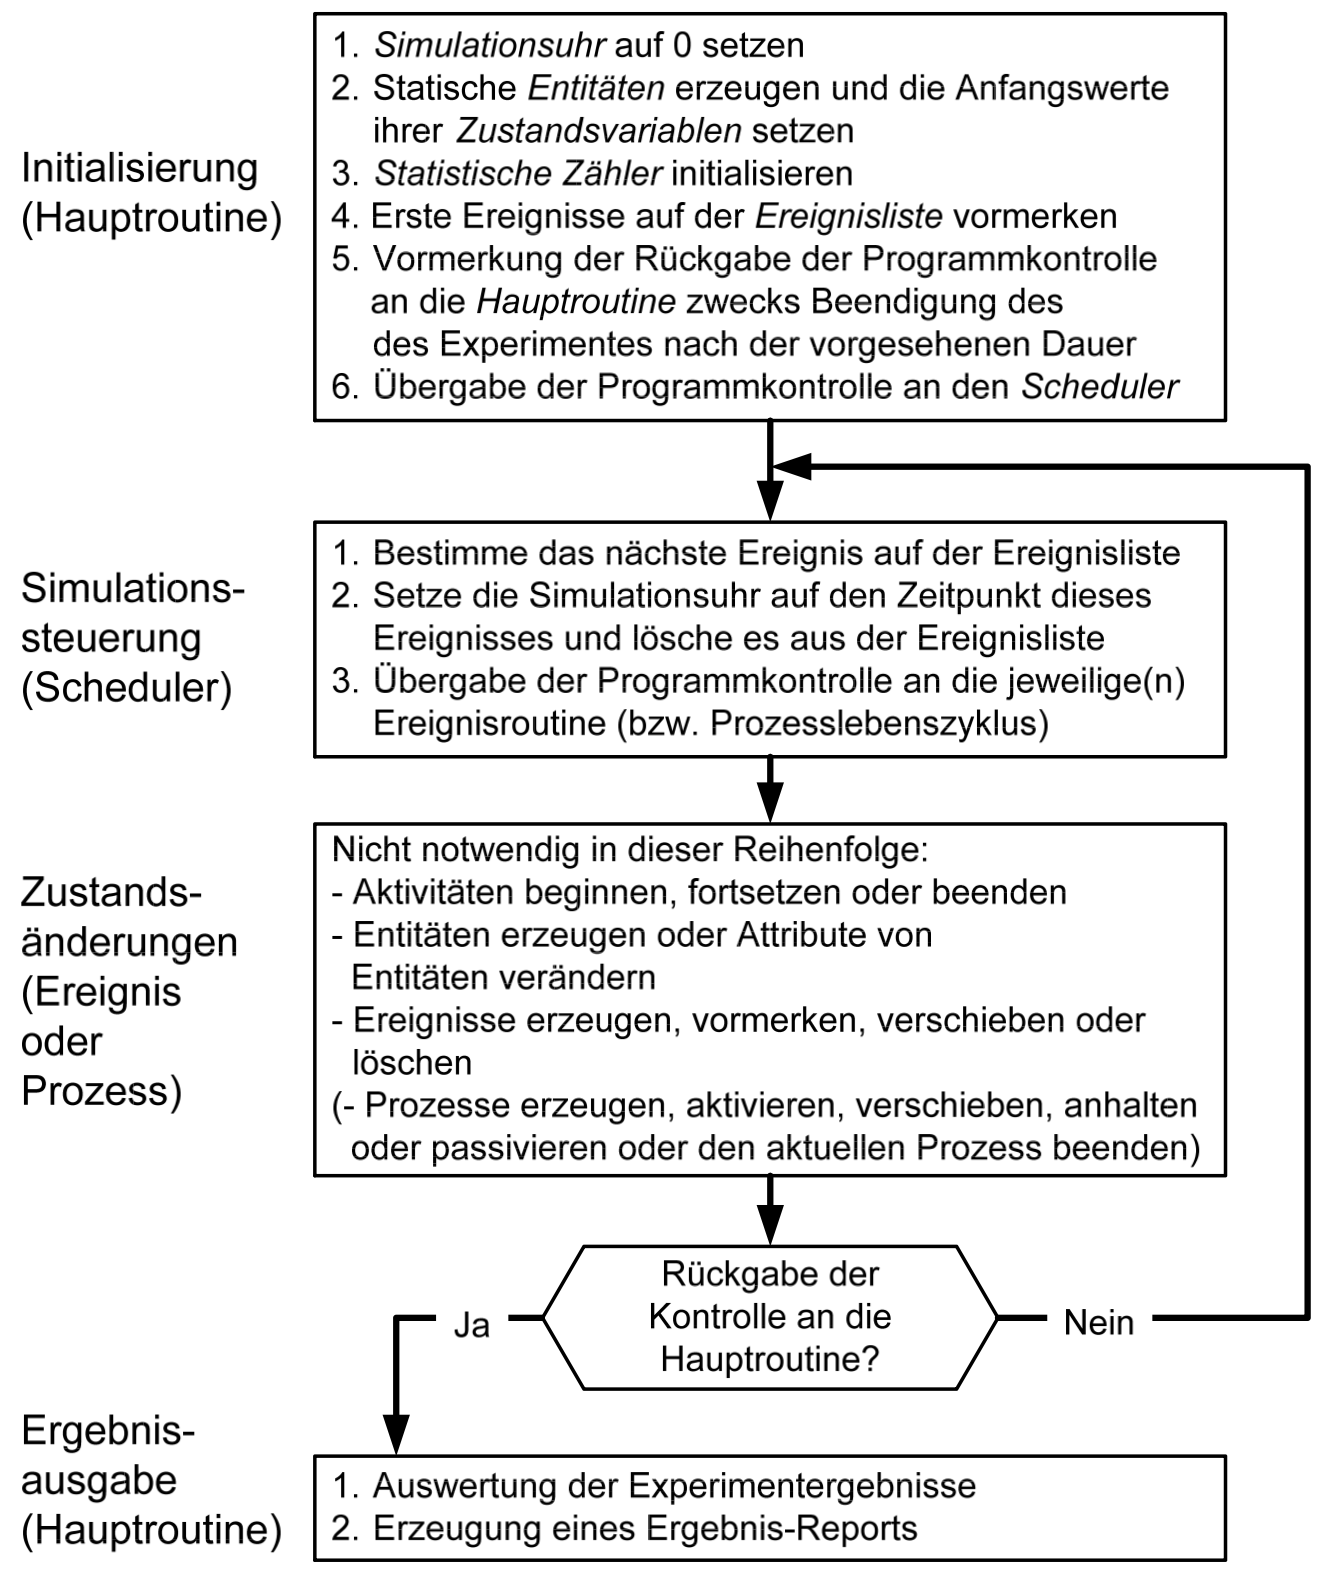
\includegraphics{res/discsim.png}
  }
  \caption{detaillierter Ablauf zeitdiskreter Simulation}
\end{figure}

\subsubsection{Prinzipielle Softwarekomponenten}
\begin{itemize}
  \item \textbf{Entitäten}: Objekte, die simuliert werden
  \item \textbf{Simulationsuhr}: Zeitverwaltung
  \item \textbf{Ereignis-/Prozessliste}: Prioritätswarteschlange
  \item \textbf{Statistikmodul}: Auswertung
  \item \textbf{Initialisierungsmethode}: Startzustand
  \item \textbf{Ereignis-/Prozessmethoden}: Verarbeitung
  \item \textbf{Hauptroutine/-prozess}: Steuerung
  \item \textbf{Auswertung-/Reportmethode}: Ergebnisse
  \item \textbf{Scheduler}: interne Simulationssteuerung
\end{itemize}

\subsection{Übersicht alternativer Modellierungsstile}
\begin{enumerate}
  \item \textbf{Ereignis}: Zustandsänderung(en) (endogen/exogen) zu einem Zeitpunkt vorgegeben
  \item \textbf{Aktivität}: Menge von Operationen innerhalb von Zeitintervall
  \item \textbf{Prozess}: Folge von Aktivitäten einer Entität über Zeitspanne
\end{enumerate}

\subsubsection{Modellierungsstile}
\begin{itemize}
  \item \textbf{Ereignisorientiert}: Zustandsänderungen einzelner Entitäten
  \item \textbf{Prozessorientiert}: beschreibt Lebenszyklen von Entitäten
  \item \textbf{Aktivitätsorientiert}: Entitäten als passive Objekte, Stationen führen Aktivitäten durch
  \item \textbf{Transaktionsorientiert}: Entitäten fordern Transaktionen (welche evtl. nicht verfügbar sind)
\end{itemize}

\subsection{Ereignisorientierte Simulation}
\begin{quote}Abbildung dynamischen Systemverhaltens durch diskrete Ereignisfolgen ("Vogelperspektive").\end{quote}

\subsubsection{Vorgehensweise bei konzeptueller Modellierung}
\begin{enumerate}
  \item \textbf{Objekte}: Identifikation von permanenten \& Modellentitäten mit Attributen
  \item optional (bei komplexen Modellen): \textbf{Zustände/Übergänge}: zB. durch Zustandsdiagramme
  \item \textbf{Zustandsänderungen}: Identifikation der Systemzustandsänderungen \& deren Zuweisung zu Entitäten
  \item \textbf{(Semi-)Formale Spezifikation}: Ereignistypen, Verhalten bei Gleichzeitigkeit
\end{enumerate}

\subsubsection{Softwaretechnische Umsetzung}
\begin{itemize}
  \item \textbf{Ereignismethoden}: Zustandsänderungen, Attributs-, Entitäts-, Ereignisverwaltung
  \item \textbf{Scheduler}: Ablaufkontrolle, sequenzielle Abarbeitung der Ereignisliste, Fortschalten der Simulationsuhr, ordnungsrichtige Ausführung der Ereignisse
\end{itemize}

\subsubsection{Unified Modeling Language UML}
\begin{quote}Standardisierte Modellierungssprache für objektorientierte Systeme mit verschiedenene Diagrammen (Perspektiven).\end{quote}

\begin{itemize}
  \item \textbf{Strukturdiagramme}: Klassendiagramme, ggfs. Packagediagramme
  \item \textbf{Verhaltensdiagramme}: Zustandsdiagramme, ggfs. Aktivitätsdiagramme
\end{itemize}

\subsection{Prozessorientierte Simulation (process interaction simulation)}
\begin{quote}Abbildung von Entitätenlebenszyklen durch Prozessmodelle ("Froschperspektive").\end{quote}

\subsubsection{Vorgehensweise}
\begin{enumerate}
  \item \textbf{UML-Zustandsdiagramme}
  \item \textbf{Identifikation der Ereignis-/Prozesstypen}
  \item \textbf{Beschreibung der Modelldynamik}: zB. BPMN
\end{enumerate}

\subsubsection{Eigenschaften bzw. Phasen}
Übergänge zwischen Phasen durch Ereignisse (interne Abbildung von Prozessen), wobei stets nur ein aktiver, aber beliebig viele passive Prozesse existieren.
\begin{enumerate}
  \item \textbf{aktiv}: zeitverzugslos, Programmkontrolle
  \item \textbf{passiv}: Zeitverbrauch, Ereigniskontrolle
        \begin{itemize}
          \item \textbf{passives Warten}: Prozess ist passiviert, auf unbestimmte Zeit, bis er extern wieder aktiviert wird
          \item \textbf{zeitkonsumierende Tätigkeit}: Prozess ist angehalten, auf bestimmte Zeit, bis er intern (automatisch) wieder aktiviert wird
        \end{itemize}
\end{enumerate}

\subsubsection{Simulationsablaufsteuerung}
\begin{itemize}
  \item \textbf{Generieren}: Erzeugung von Prozessen
  \item \textbf{Reaktivieren}: Wiederaufnahme passivierter Prozesse
  \item \textbf{Verzögern}: Verschiebung des Beginns aktiver Phasen anderer Prozesse (aus interner Ereignisliste)
  \item \textbf{Unterbrechen}: Unterbrechung eigener Aktivphase
  \item \textbf{Modifizieren}: Änderung von Objektattributen
  \item \textbf{Terminieren}: Beenden von Prozessen
\end{itemize}

\subsubsection{BPMN2.0}\label{subsec:bpmn}
\begin{itemize}
  \item \textbf{Geschäftsprozess}: Sequenzen von dem Geschäftszweck dienenden, wiederkehrenden Aktivitäten
  \item \textbf{Geschäftsprozessmanagement}: technische Implementation, Controlling/Monitoring, Dokumentation, Verbesserung
  \item \textbf{Geschäftsprozessmodellierung}: Dokumentation, Kommunikation, Kontrolle
\end{itemize}

\subsubsection{Wieso BPMN?}
\begin{itemize}
  \item Unterstützung expliziter Modellierung aktivert und passivierter, sowie angehaltener Prozesse
  \item weiter verbreitet in Wirtschaftsinformatik als zB. UML
  \item Unterstützung verschiedener Verzweigungen, Subprozesse, etc.
\end{itemize}

\subsubsection{Ausgewählte Notationselemente}
\begin{itemize}
  \item \textbf{Aktivität} (Task): Rechteck mit abgerundeten Ecken, mit Zeitverbrauch >= 0
  \item \textbf{Annotation}: Aufgabentyp (zB. Benutzer-Interaktion, Skript, …)
  \item \textbf{Zeitverbrauch als Kommentar}: in eckigen Klammern, kein offizieller Standard
  \item \textbf{Strukturelement}
        \begin{itemize}
          \item \textbf{Gateways}: zB. XOR, AND
          \item \textbf{Kontrollfluss}: Sequenz, bedingt, default/sonst
          \item \textbf{Nachrichtenfluss}: zur Synchronisation zwischen Prozessen
        \end{itemize}
  \item \textbf{Ereignis}: Kreis mit Rand, zB. Start, Ende, Zwischenereignis
  \item \textbf{Ereignisannotationen}: zB. Timer, Signale, Nachrichten
\end{itemize}

\subsection{Vergleich der Modellierungsstile}
\begin{figure}
  \centering
  \resizebox{.8\textwidth}{!}{
    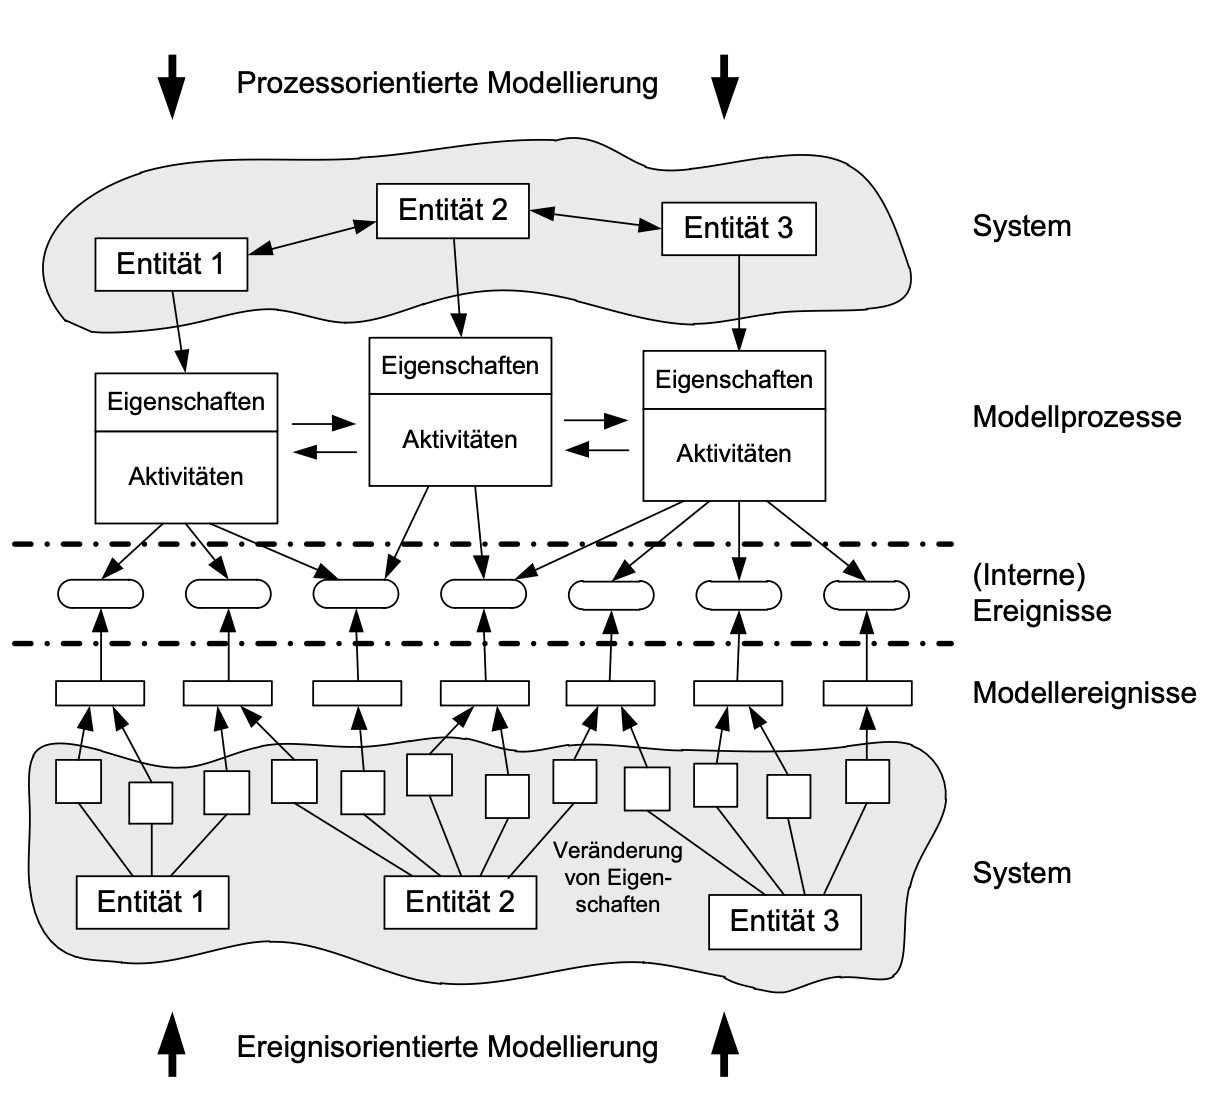
\includegraphics{res/relationship.png}
  }
  \caption{Beziehung zwischen ereignis- \& prozessorientierter Simulation.}
\end{figure}

\subsubsection{Vor- \& Nachteile der ereignisorientierten Sicht}
\begin{itemize}
  \item[+] typische Systemzustandsänderungen häufig besser durch Ereignisse zu beschreiben
  \item[+] Blick hinter die Kulissen (gleiche interne \& externe Repräsentation)
  \item[+] einfache Realisierung der Ablaufsteuerung
  \item[+] relativ effiziente Simulationsprogramme
  \item[-] Verteilung logisch zusammenhängender Abläufe auf mehrere Ereignisroutinen
  \item[-] fehleranfällig bei komplexen Systemen
  \item[$\hookrightarrow$] geeignet für einfache Systeme mit wenig Interaktion
\end{itemize}

\subsubsection{Vor- \& Nachteile der prozessorientierten Sicht}
\begin{itemize}
  \item[+] natürlichere (direktere) Modellierung
  \item[+] strukturiertere Vorgehensweise
  \item[+] größere Übersichtlichkeit
  \item[+] Verwandtschaft zur Objektorientierung
  \item[-] zT. umständlichere Modellierung
  \item[-] komplexere interne Modelle
  \item[$\hookrightarrow$] grds. vorzuziehen, in Kombination mit ereignisorientierter Sicht für Verständnis
\end{itemize}

\section{Simulationssoftware}\label{sec:simsoft}

\subsection{Typisierung}
\begin{enumerate}
  \item \textbf{Sprachebene}: Programmiersprachen, Simulationspakete/Frameworks, Simulationssprachen
  \item \textbf{Modellebene}: Fertige Modelle mit Parametrisierung
  \item \textbf{Werkzeuge}: Modellierungsfokus
\end{enumerate}

\subsubsection{Animation in der Simulation}
\begin{itemize}
  \item[+] verbessertes Testen/Validierung
  \item[+] Anschaulichkeit
  \item[+] bessere Vermittelbarkeit
  \item[-] leichte Fehlinterpretation
  \item[-] vernachlässigte Zufallsaspekte
  \item[-] oberflächliche Betrachtung
\end{itemize}

\subsection{Auswahlkriterien}
\begin{itemize}
  \item \textbf{Fachliche Angemessenheit}
        \begin{itemize}
          \item \textbf{Modellierungskonzept}: diskret/kontinuierlich, Modellierungsstile, Modellbausteine, Flexibilität, Anschaulichkeit
          \item \textbf{Anwendungsdomäne}
          \item \textbf{Experimentdurchführung}: Batch, Debugging, Optimierung
          \item \textbf{Ergebnisse \& Darstellung}: Statistiken, Grafiken, Export, Animation
          \item \textbf{Anforderungen an Nutzer}
        \end{itemize}
  \item \textbf{Technische Anforderungen}
        \begin{itemize}
          \item \textbf{Hardware/Software}: Plattform, Betriebssystem, Performanz
          \item \textbf{Integration/Schnittstellen}
          \item \textbf{Oberfläche}: GUI
        \end{itemize}
  \item \textbf{Anbietermerkmale \& Kosten}
        \begin{itemize}
          \item \textbf{Verbreitungsgrad, Referenzen, Dienstleistungen}
          \item \textbf{Weiterentwicklung}
          \item \textbf{Beschaffungs- \& Betriebskosten}
        \end{itemize}
\end{itemize}

\subsection{IYOPRO}
\begin{quote}Werkzeug gem. Typisierung, Modellierung \& Simulation mit BPMN.\end{quote}
\begin{itemize}
  \item[+] komfortable Modellerstellung: Drag \& Drop, keine Programmierkenntnisse
  \item[+] viele typische Anwendungsfälle abgedeckt, insb. Ressourcensynchronisation
  \item[+] interaktive Simulationsexperimente
  \item[+] ausführliche Simulationsreports
  \item[-] ereignis-basierte Simulation nicht möglich
  \item[-] kein Zugriff/keine Anpassung der Simulationsstruktur
  \item[-] weniger flexibel als Programmierung
\end{itemize}

\subsection{DESMO-J}
\begin{quote}Java-basiertes Simulationsframework (Sprachebene), Schwerpunkt auf Simulation\end{quote}

\section{Simulationsstatistik \& Optimierung}
\subsection{Stochastischer Modellinput}
\subsubsection{Zufallszahlenerzeugung}
\begin{quote}Verwendung für stochastische oder real zu komplexe deterministische Prozesse.\end{quote}

\begin{itemize}
  \item \textbf{Klassifizierung}
        \begin{itemize}
          \item \textbf{physikalische Zufallszahlen}: möglich (zB. Radioaktivität), aber sehr aufwändig
          \item \textbf{künstliche (Pseudo-)Zufallszahlen}: deterministisch, aber statistisch zufällig
        \end{itemize}
  \item \textbf{Methoden}
        \begin{itemize}
          \item \textbf{Lineare Kongruenzmethode}: $x_{n+1} = (a \cdot x_n + c) \mod m$
          \item \textbf{Multiplikative Kongruenzmethode}: linear mit $c=0$
          \item \textbf{Mersenne-Twister}: 32-Bit-Generator, Zykluslänge $2^{19937}-1$, gleichverteilt, effizient, moderater Speicherbedarf
          \item  \textbf{[0,1)-stetig-gleichverteilt}: Division durch Maximalwert $\text{rand}_{[0,1)} = \text{rand}_{[0,P)}()/P$
          \item \textbf{[a,b)-stetig-gleichverteilt}: durch Skalierung $\text{rand}_ {[a,b)} = a + (b-a) \cdot \text{rand}_{[0,1)]}()$
        \end{itemize}
\end{itemize}

\subsubsection{Verteilungen}

\begin{itemize}
  \item \textbf{Charakterisierung}
        \begin{itemize}
          \item \textbf{Verteilungsfunktion $F(x)$}: $F(x) = P(X \leq x)$: Wahrscheinlichkeit, dass Zufallsvariable $X$ den Wert $x$ nicht überschreitet
          \item \textbf{Dichtefunktion $f(x)$}: $f(x) = F'(x)$ bzw. $F(x) = \int_{-\infty}^x f(x) \, dx$
        \end{itemize}
  \item \textbf{Näherungsverfahren für Normalverteilung}
        \begin{itemize}
          \item \textbf{Zentraler Grenzwertsatz}: Summe von unabhhängigen, identisch verteilten Zufallsvariablen konvergiert gegen Normalverteilung
          \item \textbf{Box-Muller Methode}: $z_j = \sqrt{-2 \ln u_1} \cdot \cos(2 \pi u_2)$
          \item \textbf{Polar Methode}: Box-Muller ohne Cosinus durch Trial \& Error
        \end{itemize}
  \item \textbf{Relevante Verteilungen}
        \begin{itemize}
          \item[kont.] \textbf{Rechteckverteilung}: gleichmäßig zwischen min \& Maximalwert
          \item[kont.] \textbf{Exponentialverteilung}: Zeit bis zum Eintreten eines Ereignisses
          \item[kont.] \textbf{Normalverteilung}: Aggregation unbekannter Verteilungen
          \item[kont.] \textbf{Dreieckverteilung}: um Maximum
          \item[disk.] \textbf{Gleichverteilung}: Alternativen gleicher Wahrscheinlichkeit
          \item[disk.] \textbf{Bernoulli-Verteilung}: binär
          \item[disk.] \textbf{Binomialverteilung}: Anzahl Erfolge in $n$ Versuchen
          \item[disk.] \textbf{Geometrische Verteilung}: Anzahl Versuche bis zum ersten Erfolg
          \item[disk.] \textbf{Konstante Verteilung}: immer gleicher Wert (zB. Debugging)
        \end{itemize}
\end{itemize}

\subsection{Interpretation des stochastischen Modelloutputs}
\begin{enumerate}
  \item \textbf{Transiente (Anlauf-)Phase}: Zeit zum Einpendeln, typische Analyse nur auf diesen Bereich beschränkt (zB. wie lange dauert Boarding)
  \item \textbf{Stationäre Phase}: Zeitinvarianter Zustand, statistische Analyse möglich
\end{enumerate}

\subsubsection{Schätzgenauigkeit}
\begin{itemize}
  \item \textbf{Erwartungswert} $\bar{x} = \frac{1}{n} \sum_{i=1}^n x_i$: Mittelwert
  \item \textbf{Standardabweichung} $s = \sqrt{\frac{1}{n-1} \sum_{i=1}^n (x_i - \bar{x})^2}$: Streuung
  \item \textbf{Quantil der $T$-Verteilung} $z=1-\frac{\alpha}{2}$: bei $n < 30$
  \item \textbf{Quantil der Standardnormalverteilung} $z=1-\frac{\alpha}{2}$: bei $n \geq 30$
  \item \textbf{Konfidenzintervall} $\bar{x} \pm z \cdot \frac{s}{\sqrt{n}}$: Schätzung des Mittelwertes
\end{itemize}

\subsection{Optimierung}
\begin{itemize}
  \item \textbf{Faktor-Design}: keine eigentliche Optimierung, evtl. gut als Vorarbeit
  \item \textbf{Optimierungsproblem}: Bestimmung optimaler Parameterkonfiguration (durch exakte oder nicht-exakte Methoden)
  \item \textbf{Simulationsoptimierung}: Kreislauf aus Simulation, Optimierung
  \item \textbf{Optimierungsverfahren}: evolutionäre Methoden, lokale Suchverfahren, Monte Carlo (zufällige Suche), Neuronale Netzwerke, …
  \item \textbf{Genetische Algorithmen}: zufällige Initialisierung, Selektion, Rekombination, Mutation, Evaluation
\end{itemize}

\setcounter{section}{5}
\section{Simulationspraxis}
\subsection{Logistiksimulation}
\begin{quote}Anwendungsbereich: Planung, Steuerung, Optimierung von Material- \& Informationsflüssen.\end{quote}

\subsubsection{Logistischer Prozess}
\begin{itemize}
  \item \textbf{Materialfluss}: Aktivitätsketten zur Beschaffung, Verarbeitung oder Verteilung von Gütern (Material oder Produkte)
  \item \textbf{Informationsfluss}: Beschaffung, Übertragung, Verarbeitung, Speicherung \& Bereitstellung von Informationen zur Einleitung, Ankündigung, Begleitung und Abschluss von Materialflüssen
\end{itemize}

\subsubsection{Logistics KPIs}
\begin{itemize}
  \item \textbf{Quantitative KPIs}: Liefer-/Reaktionszeit, Lieferkosten, Umschlag/Durchsatz, Lager-/Lieferquoten, Reklamationsquote
  \item \textbf{Qualitative KPIs}: Abspracheneinhaltung, Ruf/Kundenzufriedenheit, Erreichbarkeit, Freundlichkeit
\end{itemize}


\subsection{Anforderungen an erfolgreiche Simulation}
\subsubsection{Voraussetzungen}
\begin{enumerate}
  \item \textbf{Zeitpunkt}: recht-/frühzeitig, um noch Einfluss zu nehmen
  \item \textbf{Aufwandsschätzung}: Dauer, Ressourcen, Kosten
  \item \textbf{Fachkenntnis}: Möglichkeiten/Grenzen der Simulation, Alternativen, Einblick in Realsystem, (evtl.) externe Beratung
  \item \textbf{Simulationswürdigkeit}: Sammlung/Prüfung alternativer Ansätze
  \item \textbf{Kommunikation}: zwischen Modellentwicklern \& -anwendern
  \item \textbf{Detaillierungsgrad}: ausreichend, aber nicht zu detailliert
  \item \textbf{Datenqualität}: Umfang \& Form angemessen
  \item \textbf{Simulationswerkzeug}: nach Kriterien vgl. \ref{sec:simsoft}
  \item \textbf{Validierung}: Plausibilität
  \item \textbf{Planung \& Auswertung}: Simulationslänge, Stichprobenumfang, Versuchsplanung, Schätzverfahren
  \item \textbf{Interpretation}: als statistische Werte, Berücksichtigung von Unsicherheiten, in Bezug auf Realsystem
  \item \textbf{Dokumentation}: der Einzelschritte, Aufbereitung der Ergebnisse
\end{enumerate}

\subsubsection{Projektorganisation (Rollen)}
\begin{itemize}
  \item \textbf{Entscheidungsträger}: Genehmigung, Budget, Umsetzungsentscheidung, Meetingterminierung
  \item \textbf{Projektleiter}: Deadline, QS, Budgetkontrolle, Koordination, Dokumentation, Meetings
  \item \textbf{Fachspezialisten}: Daten, Umsetzung, Meetings
  \item \textbf{Simulationsexperten}: Sofware, Modellierung, Experimente, Interpretation, Meetings
\end{itemize}

\subsubsection{Simulation als Dienstleistung}
\begin{itemize}
  \item \textbf{Make-or-Buy-Entscheidung}: interne/externe Simulation
        \begin{itemize}
          \item \textbf{Vorteile Make}: Flexibilität, Anpassung, Kontrolle, Kosten
          \item \textbf{Vorteile Buy}: Erfahrung, Unabhängigkeit, Expertenwissen, Ressourcen
        \end{itemize}
  \item \textbf{Grundleistungen}: Datenanalyse, Entwicklung, Experimente, Ergebnispräsentation, Dokumentation
  \item \textbf{Zusatzleistungen}: Datenerfassung/-beschaffung, Animation, innerbetriebliche Schulung, Beratung
\end{itemize}

\subsubsection{Kosten \& Zeitaufwand}
\begin{itemize}
  \item \textbf{Kosten}: abhängig vom Umfang (5.000€ - 100.000€), zusätzlich interne Kosten (Personal, Ressourcen)
  \item \textbf{Zeit}: kurze (2 Monate) bis lange (1 Jahr) Projekte, abhängig von Komplexität, Umfang, Datenqualität, …
  \item \textbf{Kosten bei interner Durchführung}: Softwarelizenz (1.000€ - 100.000€), Technik/Hardware (2.000€ - 25.000€), Schulung inkl. Lohnkosten (2.000€ - 25.000€), Auswahl der Simulationssoftware (5.000€ - )
  \item \textbf{Kostensenkungspotenziale}: Detaillierungsgrad/Datenbedarf, geeignetes Simulationswerkzeug, Verwendung/Weiterentwicklung von Standardmodellen, intensive Abstimmung mit Berater
\end{itemize}

\subsubsection{Typische Fehlerquellen}
\begin{itemize}
  \item \textbf{Definition}: unklare Fragestellung, fehlende Zieldefinition
  \item \textbf{Kommunikation}: unzureichend zwischen Simulationsexperten \& -anwendern
  \item \textbf{Modellierung}: unangemessen ddurch vernachlässigte Ziele, zu hohe Komplexität, unklare Grenzvorstellungen
  \item \textbf{Datenadequanz}: unzureichende Datenqualität, fehlende Daten, unklare Datenherkunft
  \item \textbf{Ergebnisinterpretation}: unangemessenes Vertrauen in Ergebnisse, Überschätzung der Gültigkeitsbereichs, fehlende Validierung
\end{itemize}

\subsubsection{Schlussfolgerungen}
\begin{itemize}
  \item \textbf{Ausschlusskriterien}: kurze Projektdauer/Zeitdruck, spätes Projektstadium, unzureichendes Know-How, umfangreiche/ständig verändernde Systeme, mangelhafte Datenlage
  \item \textbf{potenzieller Nutzen}: als Testumgebung, Vermeidung von Planungsfehlern, schnellere Entscheidungsfindung, besseres Prozesswissen/Datenlage, höheres Systemverständnis
\end{itemize}



\newpage
\part{Integrierte Software- \& Organisationsentwicklung}
\section{(IT-)Organisation \& Prozesse}

\subsection{Wertschöpfung in Unternehmen \& (Geschäfts-)Prozesse}
Wertschöpfungskette: Sequenz Ablauf von Unternehmensaktivitäten zur Schaffung eines Produktes oder einer Dienstleistung
Prozess: sachlogische Abfolge von Aktivitäten

\subsubsection{Prozesslandschaftsmodell}
\begin{enumerate}
  \item \textbf{Managementprozess}: Steuerung, Kontrolle, Planung
        \begin{itemize}
          \item Vision definieren
          \item Strategie entwickeln
          \item Strategie einführen
          \item Risiko managen
        \end{itemize}
  \item \textbf{Geschäftsprozess}: Wertschöpfungskette, primärer Zweck
        \begin{enumerate}
          \item Material beschaffen
          \item Produkt erstellen
          \item Produkt vermarkten
          \item Produkt versenden
          \item Kundenservice managen
        \end{enumerate}
  \item \textbf{Supportprozess}: Unterstützung der Geschäftsprozesse, sekundärer Zweck
        \begin{itemize}
          \item Personal managen
          \item Informationen managen
          \item Vermögenswerte managen
        \end{itemize}
\end{enumerate}

\subsubsection{Beispiele für Unternehmensprozesse}
\begin{itemize}
  \item \textbf{Quote-to-Order} (Q2O)
  \item \textbf{Order-to-Cash} (O2C)
  \item \textbf{Issue-to-Resolution} (I2R)
  \item \textbf{Application-to-Approval} (A2A)
  \item \textbf{Procure-to-Pay} (P2P)
\end{itemize}

\subsubsection{Prozessarchitekturebenen}
\begin{enumerate}
  \item Level: \textbf{Prozesslandschaft} inkl. Value Chains
  \item Level: \textbf{Geschäftsprozesse}: BPMN
  \item Level: \textbf{Subprozesse \& Aktivitäten}: BPMN
\end{enumerate}

\subsection{BPMN}

s. \ref{subsec:bpmn}

\begin{itemize}
  \item[+] graphische Darstellung
  \item[+] Überblick, Dokumentation
  \item[+] Abhängigkeiten abgebildet
  \item[+] fachliche \& technische Sicht
  \item[+] Schnittstellenanalyse
  \item[+] verschiedene Analyseverfahren
  \item[-] hoher zeitlicher Initialaufwand
  \item[-] permanenter Pflegeaufwand
  \item[-] Fokus nur auf Geschäftsprozesse
\end{itemize}

\subsection{Quantitative \& Qualitative Prozessanalyse}

\subsubsection{Qualitativ: Value-Added Analysis}
\begin{quote}Analyse der Wertschöpfungskette, um nicht-wertschöpfende Aktivitäten zu identifizieren.\end{quote}
\begin{itemize}
  \item \textbf{Value Adding}: direkter Beitrag zur Wertschöpfung
  \item \textbf{Business Value Adding}: indirekter Beitrag zur Wertschöpfung
  \item \textbf{Non-Value Adding}: keine Wertschöpfung
  \item[$\hookrightarrow$] alternativ: Root-Cause oder Stakeholder Analysis
\end{itemize}

\subsubsection{Quantitativ: Flow Analysis}
\begin{quote}Analyse der Prozessdurchlaufzeiten, um Engpässe zu identifizieren.\end{quote}
\begin{itemize}
  \item \textbf{Cycle time} (CT): Zeit von Anfang bis Ende eines Prozesses ($CT = WT + PT$)
  \item \textbf{Processing time/Theoretival cycle time} (PT/TCT): Zeit, die zur Bearbeitung benötigt wird
  \item \textbf{Waiting time} (WT): Zeit von non-value adding Aktivitäten
  \item \textbf{Cycle time efficiency} (CTE): processing time compared to cycle time ($\frac{PT}{CT}$)
  \item[$\hookrightarrow$] alternativ: Queues oder Simulation
\end{itemize}

\section{Komplexe Informationssysteme}

\section{Digital Leadership \& Business Strategy}


\end{document}